Nous désirons déplacer le robot en lui fournissant un position de destination absolue $(x, y, z)$ dans un repère lié à la salle. Or, le robot se positionne en utilisant les valeurs angulaires que doivent prendre ses moteurs. Il était donc nécessaire d'implémenter un module permettant de passer d'une position absolue aux valeurs angulaires associées, d'où la nécessité du calcul d'un modèle géométrique inverse. Ceci est intégré dans la partie "Calcul d'Impact" dans le découpage de notre application.

\subsection{Modélisation}

Afin de modéliser le bras, nous avons nommé les moteurs comme indiqué sur la photographie \ref{moteurs} :\\

\begin{figure}[!htc]
	\begin{center}
		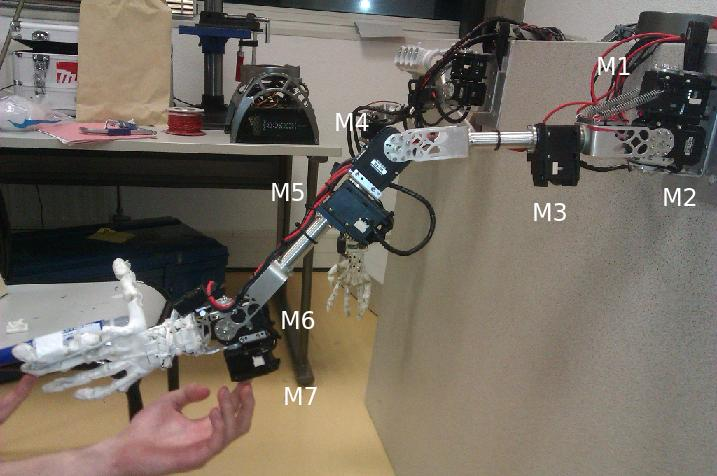
\includegraphics[scale=0.6]{images/robot1.jpg}
		\caption{Bras robotique et noms des moteurs} 
		\label{moteurs}
	\end{center}
\end{figure}

La première étape de la modélisation a été de mettre en place une paramétrisation de Denavit-Hartenberg, qui nous permet de déterminer un repère différent lié à chacun des moteurs, afin de pouvoir récupérer ensuite des équations exploitables pour la détermination du modèle géométrique inverse.
\newpage
La représentation en question est en figure \ref{denavit} :\\

\begin{figure}[!htc]
	\begin{center}
		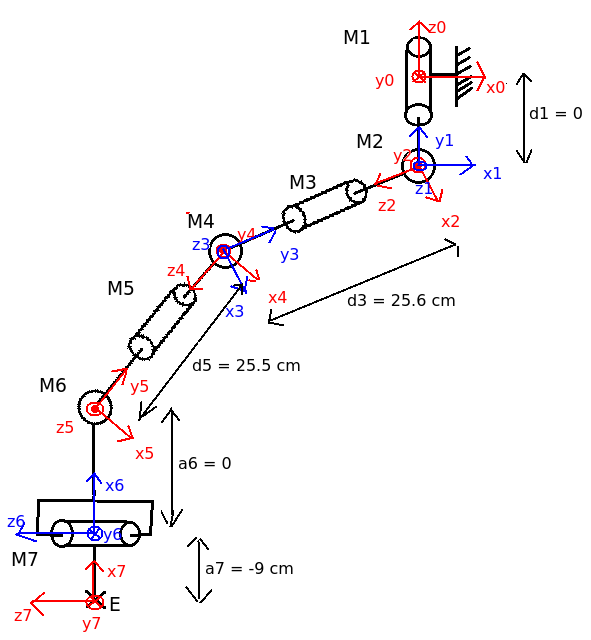
\includegraphics[scale=0.7]{images/denavit.png}
		\caption{Représentation du bras en paramétrisation de Denavit-Hartenberg} 
		\label{denavit}
	\end{center}
\end{figure}

Sur cette représentation, le point E représente la position de l'effecteur, au centre de la main robotique, point que nous voulons être celui à réceptionner la balle. Nous avons arbitrairement décidé de la valeur de sa distance au moteur 7.\\

Le repère R0 représente le repère lié à la salle. Pour des raisons de clareté, il a été représenté au centre du moteur 0, néanmoins, dans la paramétrisation de denavit Hartenberg, seul l'orientation de son axe z est imposé. Nous avons donc fais le choix de placer son origine au centre du moteur M2, ce qui nous permettra de simplifier nos équations en forçant ainsi $d1 = 0$.\\

Une fois cette représentation effectuée, et ces repères placés, nous sommes en mesure d'établir le tableau de Denavit-Hartenberg suivant :\\

\begin{tabular}{|c|c|c|c|c|}
\hline
i, i+1 & $Rot_{zi}$ & $Trans_{xi+1}$ & $Trans_{zi}$ & $Rot_{xi+1}$\\
\hline   
0, 1 & $\theta_1^*$ & / & d1 = 0 & $+90^o$        \\
1, 2 & $\theta_2^*$ & / & / & $+90^o$\\
2, 3 & $\theta_3^*$ & / & d3 = 26.5 cm & $-90^o$\\
3, 4 & $\theta_4^*$ & / & / & $+90^o$\\
4, 5 & $\theta_5^*$ & / & d5 = 25.5 cm& $-90^o$\\
5, 6 & $\theta_6^*$ & a6 = 0 & / & $+90^o$\\
6, 7 & $\theta_7^*$ & a7 = -9 cm & / & / \\
\hline
\end{tabular}

Une fois cette représentation terminée, nous pouvons commencer l'implémentation de la détermination d'un modèle géométique inverse.

\subsection{Détermination des équations du modèle géométrique inverse}

Afin de déterminer un modèle géométrique inverse, la première étape a été de trouver et de définir les équations à résoudre permettant d'obtenir les valeurs angulaires à prendre sur les moteurs pour correspondre à une position et une orientation fixée de la main.\\

Pour ce faire, nous avons utilisé le logiciel libre de calcul formel Maxima, dans lequel nous avons défini les matrices de transformations homogènes associées au bras grâce à notre représentation de Denavit-Hartenberg, ainsi qu'une matrice de positionnement et d'orientation désirée de la main dans le repère 0, qui correspond à la position et à l'orientation de la main que l'on souhaite obtenir, et qui s'écrira avec le triplet $(x, y, z)$ qu'un modèle d'interpolation avec le module de prédiction de trajectoire fournira.\\

Constatons que pour une orientation et une position fixée de la main, bien qu'il y ait une infinité de positions du bras qui soient compatibles, la valeur de l'angle du moteur 4 reste elle toujours identique. De plus, nous savons que la distance entre le centre du moteur 2 et le centre du moteur 4 est fixe, dépendante des caractéristique du robot, égale à d3. Il en va de même pour la distance entre les centres des moteurs 4 et 6, qui vaut d5.\\

De plus, pour une position et une orientation fixe de la main, le centre du moteur 6 est lui aussi déterminé, et immobile dans le repère 0. Le centre du moteur 2 étant l'origine de ce repère 0, la position désirée de l'effecteur nous donne connue la position du centre de ce moteur 6, et donc la distance entre les centres des moteurs 2 et 6.
\newpage

Nous avons donc ainsi un triangle formé par les centres des moteurs 2, 4 et 6, dont nous connaissons les longueurs et côtés, ce qui nous permet ainsi de déterminer la valeur de l'angle du moteur 4 selon les paramètres imposés par la position désirée de la main.\\

Arrivé à ce niveau la, nous avons donc 6 valeurs à déterminer, pour lesquelles nous avons 1 degré le liberté. Nous faisons le choix arbitraire d'imposer la valeur du moteur 3 (choisi du fait que le moteur 5 permet une liberté suffisante dans le déplacement malgré une immobilisation du moteur 3), ce qui nous fige le système.\\

Après quoi, nous utilisons maxima pour obtenir des équations sur les angles des moteurs restants. Ainsi, nous pouvons déterminer (toujours en fonction des coordonnées désirées de la main) des équations nous permettant d'avoir la valeurs des angles restant en recherchant et en exprimant les égalités suivantes avec Maxima :\\

\begin{itemize}
\item $\theta_4$ est connu, déterminé précédemment via la méthode du triangle.
\item $\theta_3$ est fixée arbitrairement.
\item L'expression de l'égalité $O_{2, 6} = T_{2, 0} . Od_{0, 6}$ nous donne deux équations de Paul de type 2 nous permettant de déterminer respectivement $\theta_1$ et  $\theta_2$
\item L'expression de l'égalité $T_{4, 7} = Td_{4, 7}$ nous permet enfin de récupérer trois équations qui nous donneront les valeurs de $\theta_5$, $\theta_6$ et $\theta_7$\\

\end{itemize}

Nous avons donc, à ce niveau, fixé arbitrairement la valeur de M3, et obtenu six équations nous permettant de déterminer les valeurs des moteurs restants.

\subsection{Résolution des équations du modèle géométrique inverse}

Nous avons ensuite entamé l'implémentation d'un module du code C++ qui nous permettra de résoudre ces équations, afin d'obtenir les valeurs angulaires à passer effectivement au robot afin que la main se place dans une position $(x, y, z)$ voulue.\\

Les équations à résoudre par ce module sont toutes des équations de Paul de type 2 ou des équations triginométriques qui auront toutes, dans le cas ou l'équation est bien posée et dans le cas général, deux solutions distinctes. Ces deux solutions seront mathématiquement correctes, mais seule une sera applicable sur le robot. Ainsi, il est necéssaire pour ce module de tester les valeurs renvoyées par les fonctions de résolution d'équations afin de savoir quelle valeure garder, et pour ce faire, de récupérer toutes les valeurs minimales et maximales pouvant être atteintes par les différents moteurs composant le bras.
